\chapter{3D Model Building}
This chapter describes how to build a generative textured 3D face model from an example set of 3D face scans. A morphable model is derived from the set of scans by transforming their shape and texture into a vector space representation. The term generative implies that - as the face space is spanned by the set of examples - new faces can be generated by calculating linear combinations of these examples. 

\section{3D Morphable Model}
The 3D Morphable Model (3DMM) published by Blanz and Vetter in 1999 (bib) is a multidimensional function for modelling textured faces derived from a large set of 3D face scans. 
A vector space of face shapes can be constructed from the available data set where each face is represented by a shape-vector $S \in \mathbb{R}^{3n}$ that consists of a component-wise listing of its $n$ vertices. The texture-vector then $T \in
\mathbb{T}^{3n}$ contains the corresponding RGB values in similar fassion.
New shapes and textures can now be constructed/conceived through a linear combination of the set of $m$ available faces governed by shape and texture coefficients $\vec\alpha, \vec\beta \in \mathbb{R}^{m}$.
\begin{equation}
\label{eq:MM}
\mathcal{S}_{new}=\sum_{i=1}^{m}\alpha_{i}S_{i}, \quad \mathcal{T}_{new}=\sum_{i=1}^{m}\beta_{i}T_{i}
\end{equation}
However, the goal of such a 3D face model is not just to construct arbitrary faces with linear combinations of the set of examples, but to derive plausible faces from them. This is achieved by estimating two multivariate normal distributions for the coefficients in $\vec\alpha$ and $\vec\beta$.
These multivariate normal distributions are constructed from the average face shapes $\overline{S} \in \mathbb{R}^{3N}$ and textures $\overline{T} \in \mathbb{R}^{3N}$ of the datasets and the covariance matrices $K_{S}$ and $K_{T}$, which are defined over the residuals of each example and with both the shape $R_{S}=S-\overline{S}$ and texture $R_{T}=T-\overline{T}$ averages. The covariance matrices are then used to perform two Principal Component Analysis (PCAs)
which define basis transformations to two orthogonal coordinate systems the axis of which are the eigenvectors of the respective covariance matrices.
\begin{equation}
\label{eq:MM}
\mathcal{S}(\vec\alpha)=\overline{S}+S\vec\alpha, \quad \mathcal{T}(\vec\beta)=\overline{T}+T\vec\beta
\end{equation}
In \eqref{eq:MM} the $N=m$ principal eigenvectors of $K_{S}$ and $K_{T}$ respectively are assembled column-wise in S and T and scaled in a way such that the prior distribution over the face shape and texture parameters is given by a multivariate normal distribution with unit covariance (Amberg).
\begin{equation}
    p(\vec\alpha, \vec\beta) = \mathcal{N}(\vec\alpha\vert|\vect{0}, \mathbb{I})\mathcal{N}(\vec\beta\vert|\vect{0}, \mathbb{I})
\end{equation}
By observing the likelihood of the coefficients it is now possible to find out how likely/admissible/plausible the appearance of a corresponding face is.
\viscomment{likelihood of the faces p(faces | unknown parameter values) OR what are the most likely parameters given the available set of faces}

\section{Achieving Correspondence through Registration}
In order for a 3D Morphable Model to generate plausible faces we have to make sure that all faces share the same representation, so that only the same parts of the respective faces are combined with oneanother, for example a nose is combined with another nose and not with a mouth. For this reason, the meshs first have to be brought into correspondence. In fact, we need dense correspondence between all mesh points. This is the case when vertices at the same semantical position in
different meshs, i.e the left corner of the left eye, have the same vertex number. The process of calculating a dense point-to-point correspondence between two meshs is called registration.  
\begin{comment}
meaning that all faces share the same mesh triangulation, respectively the vertices at the same semantical position, i.e. the corner of the eye, have a similar vertex number. Correspondence is achieved/accomplished through the process of registration.
\textit{Now in order to obtain a 3D representations of the face we need to transform a template face so that it fits a particular 3D face scan. To find the transformation, however, we first have to find feature points in both 3D representations which correspond to the same semantical structure. Previous work has shown that point landmarks are not sufficient to preserve the level of detail which is imminent in the regions of the eyes, ears and lips and that the computed
transformations are not able to preserve these regions. For this reason, additional line features have been introduced. In order to relate these}
\end{comment} 
The training data used for learning a 3D Morphable Models consists solely of registered examples of the 3D shape and texture of faces.

\paragraph{Registration Algorithm}
When performing registration, we start with a template shape that is a prototype of the semantic parametrization that should be established for all data sets (Prototype created manually?). In order to compute the parametrization for another shape we deform the template to match this shape, which is then referred to as the target. Both are considered as matched if the semantic points are mapped onto each other satisfying a specified similarity measure. If a dense point-to-point
correspondence is achieved, the target shape can be replaced with the deformed template, which will further be used in the process of building a model.\\
A registration algorithm uses prior information in the form of manually clicked feature points at prominent points of the face, so called landmarks, on all of the face meshs for the purpose of computing an accurate deformation. Correspondence in-between these points is defined through smooth deformations of the template mesh which match the surface and feature points of the target. 
In this thesis we present a registration algorithm which is novel to the problem of 3D face registration in two ways: the deformation is modeled using Gaussian Process Regression, a
method from the field of Machine Learning and the use of prior information is extended to parametric curves marking complex regions of the face, refered to as line features. 

\section{Available Data}
For testing the registration algorithm we have given a set of about 300 face scans - male as well as female - all of them recorded at the University of Basel by an active stereo vision system with light sources and structured light, engineered by the company ABW-3D. The scanner records four 3D surfaces, called shells, for every face and further records three high resolution color images. 
\begin{SCfigure}[][h!]
\centering
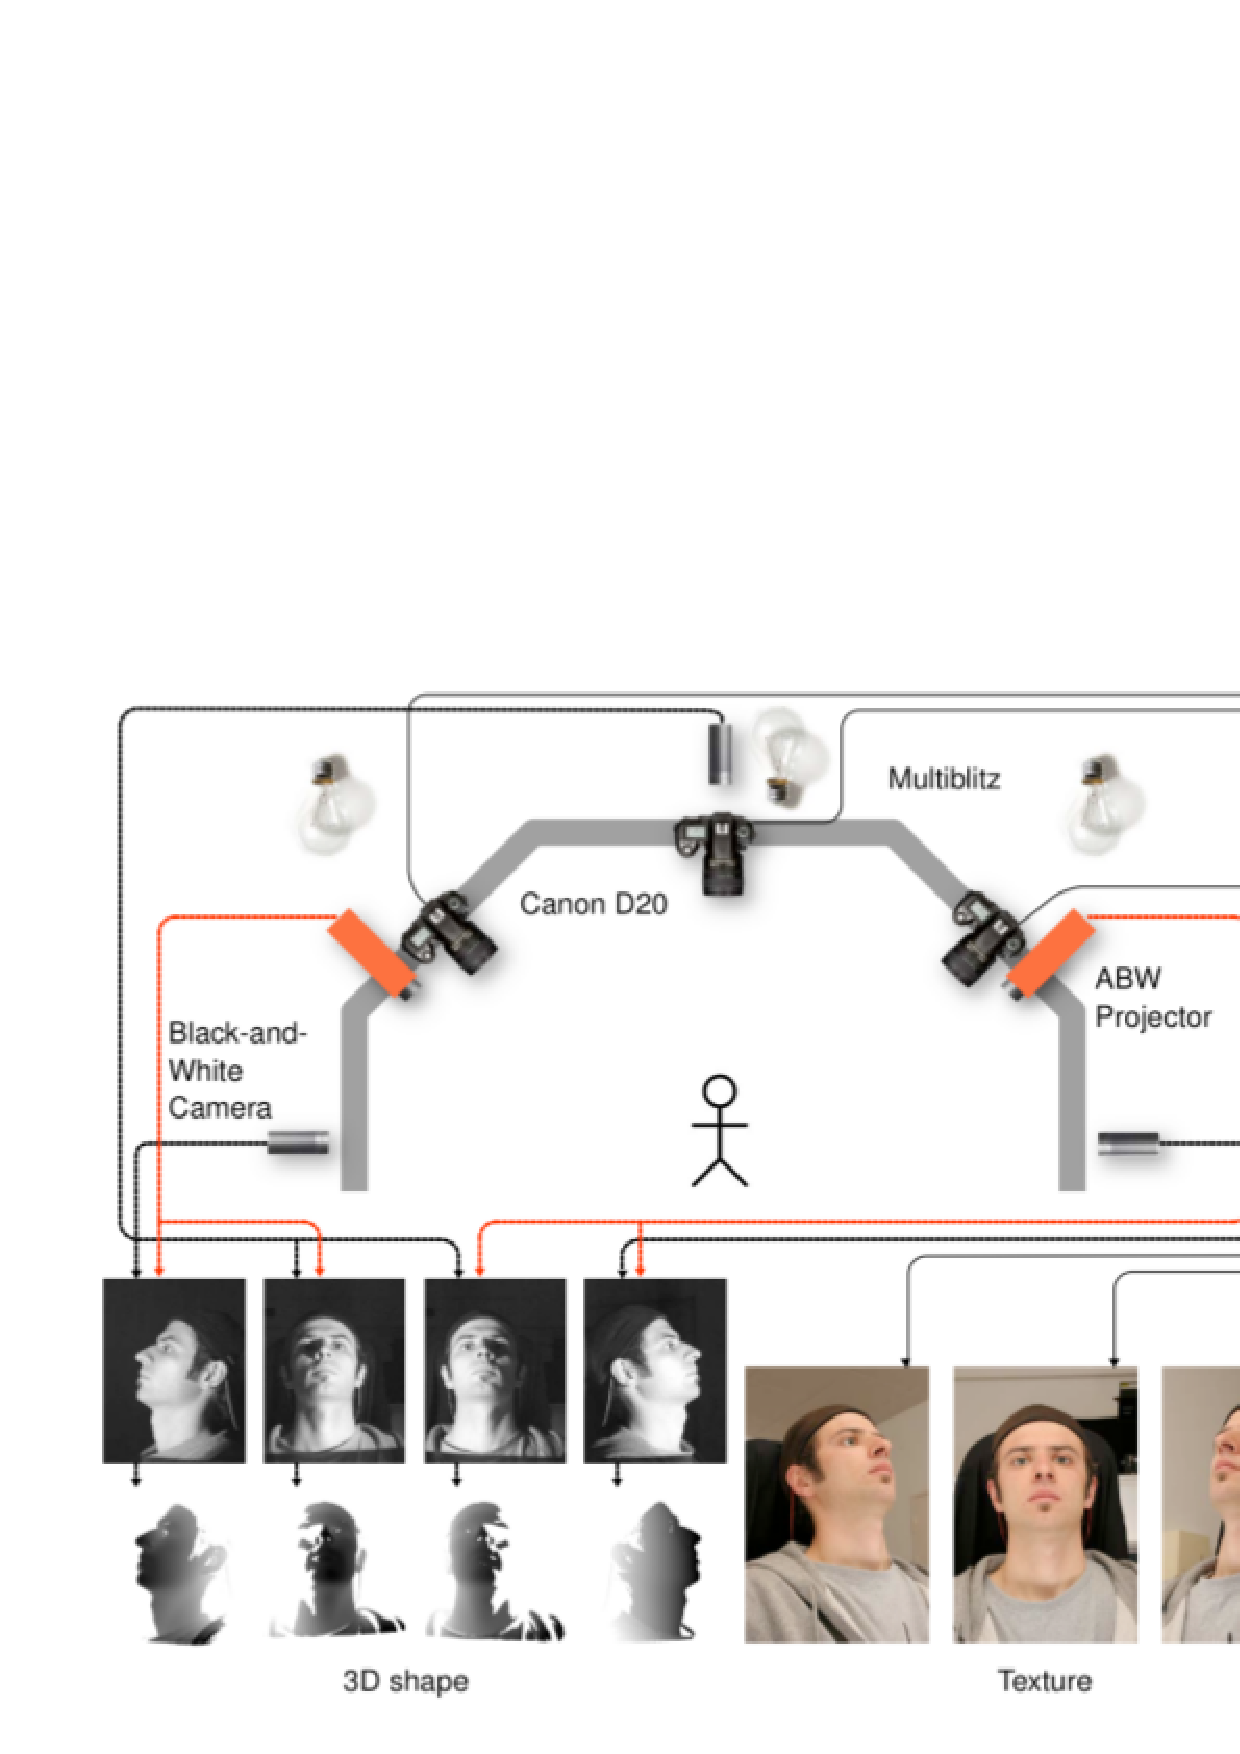
\includegraphics[width=0.7\textwidth]{./resources/figures/scanner.pdf}
\caption{schema of the structured light 3D scanning system employed to record the facial scans. It consists of two projectors that project triangle gradient patterns on to a face from opposing angles, three black-and-white cameras used for the triangulation and three digital cameras which record the facial skin.}
\label{fig:scanner}
\end{SCfigure}
The scan data consists of four seperate 3D surfaces, called shells, and three high resolution
images for the texture of the skin. The 3D shells are obtained through triangulation.
Each of the four black-and-white cameras records the triangle gradient patterns - stripe patterns - emitted from the two projectors. The patterns allow for the extraction of depth information by the four neighbouring projector-camera-pairs using triangulation.  
The eyes and hair can not be captured due to their reflection properties. Therefore the shells only cover the front and the side of the head and have holes in the eyes and instead of parts of the ears. 
\begin{figure}[h!]
    \subfloat[3D shells]{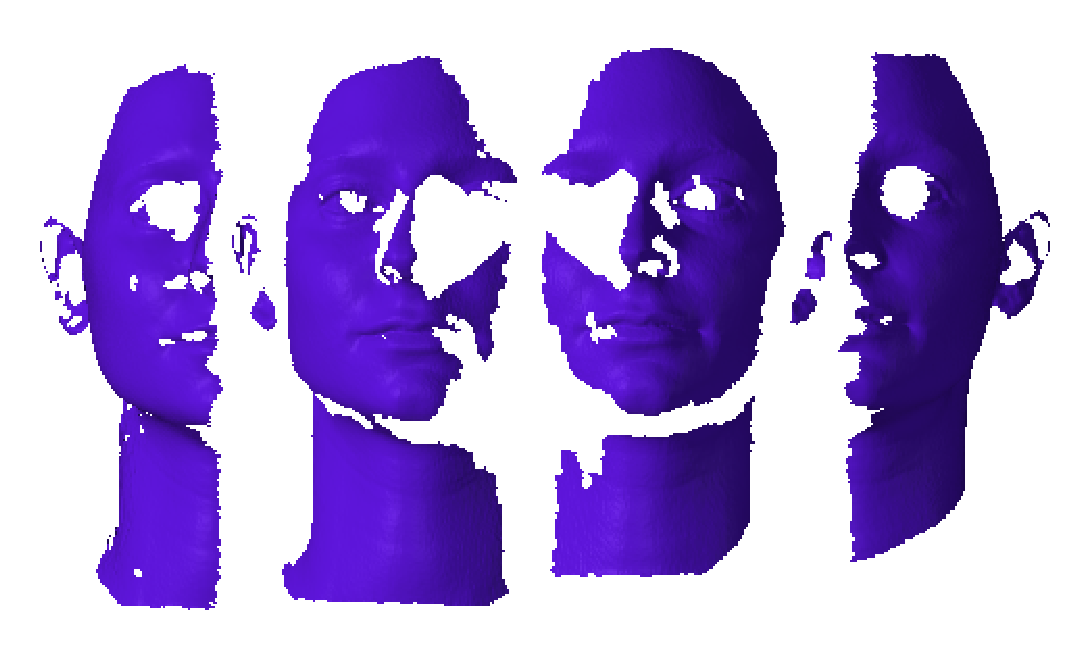
\includegraphics[width=.7\textwidth]{./resources/figures/shells.eps}}
    \subfloat[merged shells]{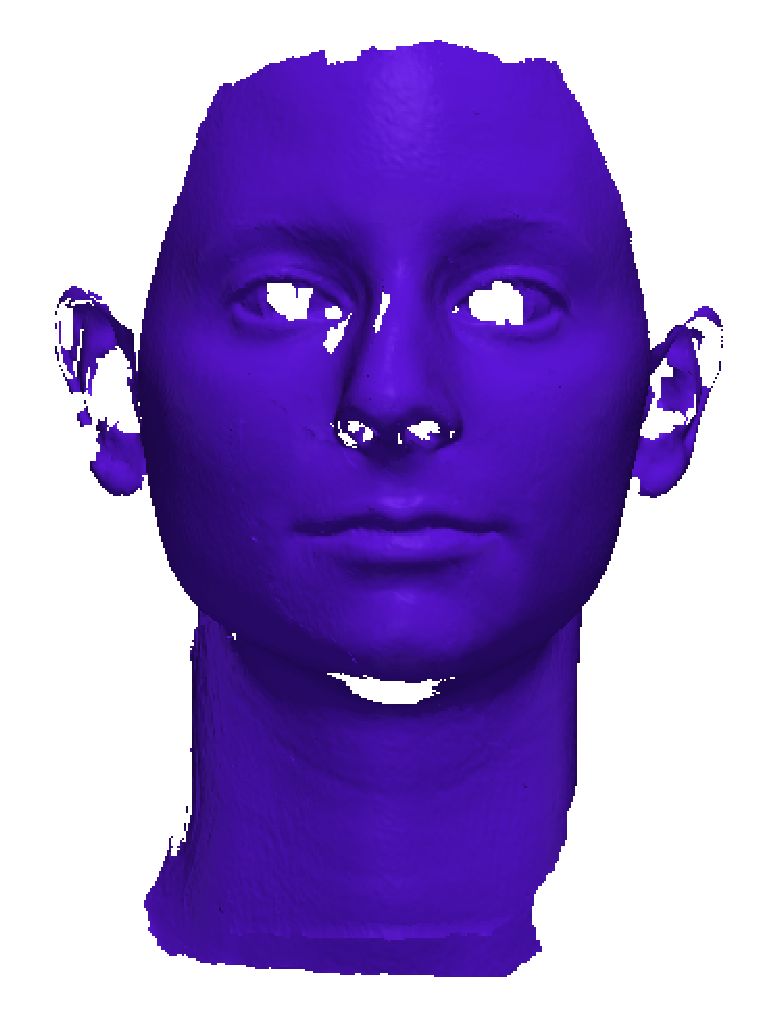
\includegraphics[width=.3\textwidth]{./resources/figures/scan.eps}}
\caption{\ldots}
\label{fig:scan}
\end{figure}

\viscomment{show shells}
To obtain a whole mesh the 3D shells first have to be cleaned and then merged.
Additionally to the scans, we use manually annotated data. A set of prominent points, so called landmarks, was given for every face. 
\begin{wrapfigure}{r}{.4\textwidth}
    \centering
    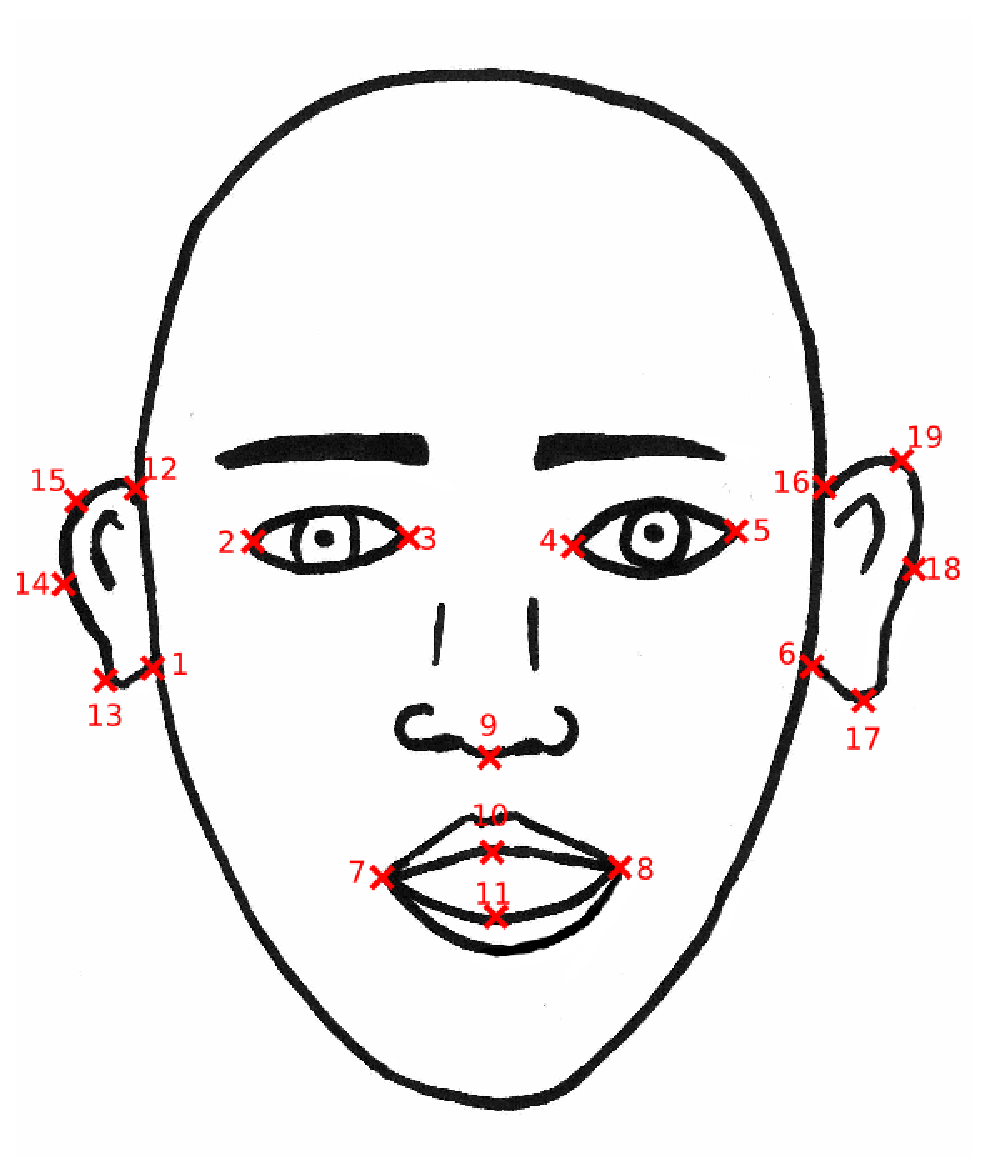
\includegraphics[width=.3\textwidth]{./resources/figures/schema_marked.eps}
\end{wrapfigure}
\viscomment{show landmarks}
\viscomment{How express that landmarks were created after feature points to enhance registration?}
Furthermore, we use the color images to create 2D parametric curves that describe key regions of the face, i.e. the eyes. The line features will be fully introduced together with the registration pipeline. In the next chapter we will elaborate on the approach of using Gaussian Processes to solving the problem 3D face registration and then describe how to incorporate the annotations.
\begin{comment}
From these scans we want to create fully textured 3D faces, which can be used to build a new face model.
\end{comment}
